\chapterauthor{Vehicle Dynamics Simulation}{Harry Emes}
% =====================================================================

% ---------------------------------------------------------------------
\section{Introduction}
\label{sec:intro}
% ---------------------------------------------------------------------

The Formula Student Acceleration Event (FS-D~5) is a \SI{75}{\metre}
standing start; for EVs, FS-EV~2.2 caps electrical power drawn from the
accumulator at \SI{80}{\kilo\watt}, and FS-D~5.3.1 disqualifies runs
over \SI{25}{\second}. A competitive configuration must be
traction-limited at launch and power-limited later while respecting
the power cap and avoiding front-axle lift; mass, centre of gravity,
tyres, gearing, drivetrain efficiency, and electrical architecture are
owned elsewhere in this report. A quantitative, rules-aware longitudinal
simulation is used to rank design levers, reject configurations that
breach FS-EV~2.2 or FS-D~5.3.1 before hardware commitment, predict the
final agreed vehicle, and apportion margin across chapters.

This chapter presents simulation methodology
(Section~\ref{sec:methodology}); verification
(Section~\ref{sec:vv}); sensitivity and optimisation
(Section~\ref{sec:sensitivity}); and predicted performance for the
final configuration (Section~\ref{sec:final_run}).

% ---------------------------------------------------------------------
\section{Simulation Methodology}
\label{sec:methodology}
% ---------------------------------------------------------------------

The simulation solves a four-state longitudinal model
($\mathbf{x} = [x, v, \omega_{w,f}, \omega_{w,r}]^\top$) on a
\SI{1}{\milli\second} timestep, computing tyre, aerodynamic, rolling
and drive forces at each sub-step of a fourth-order Runge--Kutta
integrator. Weight acts at the centre of gravity; aerodynamic drag and
downforce follow from velocity; quasi-static load transfer yields
per-axle normals; the Pacejka tyre model maps normal load and slip to
tractive force; and the powertrain supplies rear wheel torque subject to
the FS-EV~2.2 electrical power limit. Net longitudinal force advances the
state via RK4. Each following subsection specifies one component of this
balance.

% ---------------------------------------------------------------------
\subsection{Longitudinal equation of motion and effective mass}
\label{sec:eom}
% ---------------------------------------------------------------------

Newton's second law applied longitudinally to the vehicle centre of
mass gives

\begin{equation}
\left(m_v + \frac{4 I_w}{r_w^2}\right) a = F_x - F_\text{drag} - F_\text{rr},
\label{eq:eom}
\end{equation}

where $m_v$ is the vehicle mass including driver, $I_w$ is the
rotational inertia of a single road wheel about its spin axis, $r_w$
is the loaded wheel radius, $a$ is the longitudinal acceleration,
$F_x$ is the net tractive force at the contact patch, and
$F_\text{drag}$ and $F_\text{rr}$ are aerodynamic drag and rolling
resistance. The $4 I_w / r_w^2$ term is the translational mass
equivalent of the rotational inertia of four wheels. For the baseline
vehicle ($m_v = \SI{200}{\kilo\gram}$,
$I_w = \SI{0.10}{\kilo\gram\metre\squared}$,
$r_w = \SI{0.247}{\metre}$), this contributes
$4 I_w / r_w^2 = \SI{6.5}{\kilo\gram}$, a \SI{3.3}{\percent}
effective-mass penalty. It is small but non-negligible over a
\SI{75}{\metre} event and is retained throughout the analysis.

% ---------------------------------------------------------------------
\subsection{Quasi-static longitudinal load transfer}
\label{sec:load_transfer}
% ---------------------------------------------------------------------

Under longitudinal acceleration, weight transfers from the front to
the rear axle. Taking moments about the rear contact patch gives the
static rear normal force

\begin{equation}
F_{z,r}^{\text{static}} = \frac{m_v g \, (L - L_{CG})}{L},
\qquad
F_{z,f}^{\text{static}} = m_v g - F_{z,r}^{\text{static}},
\label{eq:static_normal}
\end{equation}

where $L$ is the wheelbase and $L_{CG}$ is the longitudinal distance
from the front axle to the centre of gravity. The
acceleration-induced load transfer is

\begin{equation}
\Delta F_z = \frac{m_v \, a \, h_{CG}}{L},
\label{eq:load_transfer}
\end{equation}

with $h_{CG}$ the centre-of-gravity height above the ground. Combined
with aerodynamic downforce $F_{L,f}$, $F_{L,r}$, the instantaneous
axle normal forces are

\begin{equation}
F_{z,f} = F_{z,f}^\text{static} - \Delta F_z + F_{L,f},
\qquad
F_{z,r} = F_{z,r}^\text{static} + \Delta F_z + F_{L,r}.
\label{eq:normal_forces}
\end{equation}

The wheelie onset occurs when $F_{z,f} \to 0$; in the absence of
downforce this gives

\begin{equation}
a_\text{wheelie} = \frac{F_{z,f}^\text{static} L}{m_v h_{CG}}
                 = \frac{g (L - L_{CG})}{h_{CG}}.
\label{eq:wheelie}
\end{equation}

For the baseline parameters ($L = \SI{1.60}{\metre}$,
$L_{CG} = \SI{1.14}{\metre}$, $h_{CG} = \SI{0.22}{\metre}$) this
gives $a_\text{wheelie} = \SI{20.5}{\metre\per\second\squared}$,
comfortably above the simulated peak of
\SI{12.86}{\metre\per\second\squared}.

Anti-squat (ratio $\text{AS} \in [0, 1]$, Section~\ref{sec:antisquat_dynamic_toe})
multiplies Eq.~\ref{eq:load_transfer} by $(1 - k_\text{AS})$ with
$k_\text{AS} = 0.2\,\text{AS}$. This gives a design-side lever to
retain front normal force without lowering $h_{CG}$ or lengthening
$L$.

% ---------------------------------------------------------------------
\subsection{Tyre force model}
\label{sec:tyre}
% ---------------------------------------------------------------------

The longitudinal tractive force at each driven axle follows

\begin{equation}
F_x = \mu(\kappa, F_z)\, F_z,
\qquad
\kappa = \frac{\omega_w r_w - v}{\max(|v|,\, v_\text{floor})},
\label{eq:slip_ratio}
\end{equation}

where $\kappa$ is the longitudinal slip ratio. The denominator is
floored at $v_\text{floor} = \SI{0.1}{\metre\per\second}$ to keep
Eq.~\ref{eq:slip_ratio} well-posed at standstill; below this velocity
the slip ratio is saturated to $\pm 1$ depending on the sign of
wheel velocity, which is physically reasonable for a spinning wheel
against a stationary vehicle.

Longitudinal friction coefficient $\mu(\kappa, F_z)$ is evaluated with
the Pacejka Magic Formula \cite{pacejka2012},

\begin{equation}
\mu(\kappa, F_z) = D \sin\!\Big( C \arctan\!\big( B\kappa - E(B\kappa - \arctan(B\kappa)) \big) \Big),
\label{eq:pacejka}
\end{equation}

with load-dependent peak $D = F_z (p_{Dx1} + p_{Dx2}\,\Delta F_z /
F_{z,0})$ and dimensionless stiffness factor $B = p_{Kx1} +
p_{Kx2}\,\Delta F_z / F_{z,0}$.
The coefficients used in the baseline configuration are listed in
Table~\ref{tab:pacejka}. They are derived from the Avon FSAE tyre
lateral data available to the group and typical FSAE longitudinal
characteristics reported in the literature \cite{milliken1995,
pacejka2012}, scaled to a representative slick peak friction coefficient
$\mu_\text{max} = 1.7$.

\begin{table}[H]
\centering
\caption{Pacejka Magic Formula coefficients used in the baseline
configuration. Load sensitivity is captured through $p_{Dx2}$ and
$p_{Kx2}$; the reference load $F_{z,0}$ is chosen as a typical rear
axle load during acceleration.}
\label{tab:pacejka}
\footnotesize
\begin{tabular}{|l|c|l|}
\hline
\textbf{Coefficient} & \textbf{Baseline} & \textbf{Role} \\
\hline
Shape factor $C$                & 1.65   & Controls sharpness of the peak. \\
Peak-load coefficient $p_{Dx1}$ & 1.70   & Peak friction at nominal load. \\
Load-sensitivity $p_{Dx2}$      & $-0.12$ & Peak drops by 12\% per unit $\Delta F_z / F_{z,0}$. \\
Stiffness $p_{Kx1}$             & $35\,000$ N/rad & Sets curve slope at origin. \\
Stiffness load-sens. $p_{Kx2}$  & $-3\,000$ N/rad & Widens optimal slip at high load. \\
Curvature $E$                   & $0.10$ & Shape of the post-peak roll-off. \\
Reference load $F_{z,0}$        & \SI{1500}{\newton} & Normalisation; typical rear axle load. \\
\hline
\end{tabular}
\end{table}

\subsubsection{Thermal grip window}
\label{sec:thermal}

Tyre grip is a strong function of carcass temperature. A compact
lumped thermal model is available as an optional overlay on the
Pacejka peak:

\begin{equation}
\mu_\text{peak}(T) = \mu_\text{peak,0}
\exp\!\left(-\frac{(T - T_\text{opt})^2}{2 \sigma^2}\right),
\label{eq:thermal}
\end{equation}

with $T_\text{opt} = \SI{80}{\celsius}$ and
$\sigma = \SI{60}{\kelvin}$ based on published FSAE slick data
\cite{milliken1995}. The model captures the essential effect that
cold tyres at launch ($T \sim \SI{25}{\celsius}$) operate at roughly
$0.87\,\mu_\text{peak,0}$, while well-warmed tyres
($T \sim T_\text{opt}$) deliver the full peak. The model is disabled
in the baseline runs reported here because the acceleration event is
short and the track-ready tyre temperature is set in the preceding
warm-up lap rather than by the event itself, but it is retained for
the robustness analysis (Section~\ref{sec:drywet}).

% ---------------------------------------------------------------------
\subsection{Powertrain and the electrical power limit}
\label{sec:powertrain}
% ---------------------------------------------------------------------

FS-EV~2.2 caps \textit{electrical} power at the accumulator outlet at
\SI{80}{\kilo\watt}, not mechanical power at the wheel. Limiting
motor torque alone is therefore insufficient: the same motor torque
corresponds to a range of electrical powers depending on motor speed,
drivetrain efficiency, and battery voltage.

The model represents a YASA P400R permanent-magnet motor
($K_t = \SI{0.822}{\newton\metre\per\ampere}$, peak AC current
\SI{285}{\ampere} through the BAMOCAR PG-D3 inverter
\cite{bamocar_pg, yasa_p400r}), a single-ratio reduction of
$N_g = 5.5$, a drivetrain efficiency of $\eta_\text{drv} = 0.95$, and
a \SI{600}{\volt} nominal supercapacitor bus (Section~\ref{subsec:supercapacitor_analysis}). For a
requested wheel torque $T_w^\text{req}$:

\begin{equation}
T_m = \frac{T_w^\text{req}}{N_g \, \eta_\text{drv}},
\qquad
I_m = \frac{T_m}{K_t},
\qquad
P_\text{elec} = V_\text{bus} I_m.
\label{eq:powertrain_basic}
\end{equation}

The \SI{80}{\kilo\watt} cap is enforced by clipping motor current
first and mapping back to wheel torque:

\begin{equation}
I_m^\star = \min\!\left(I_m,\; \frac{P_\text{max}}{V_\text{bus}}\right),
\qquad
T_w = K_t I_m^\star N_g \, \eta_\text{drv}.
\label{eq:power_limit}
\end{equation}

The peak motor torque is $T_m^\text{peak} = K_t I_\text{max} =
\SI{234}{\newton\metre}$, so the constraint activates at motor speed
$\omega^\star = P_\text{max}/T_m^\text{peak} = \SI{341}{\radian\per\second}$
(\num{3260} rpm), corresponding to a vehicle speed of
$v^\star = \omega^\star r_w / N_g = \SI{15.4}{\metre\per\second}$
(\SI{55}{\kilo\metre\per\hour}). Every acceleration event above this
speed is power-limited; for a \SI{75}{\metre} run reaching
\SI{33}{\metre\per\second}, more than \SI{64}{\percent} of the run
time is spent in the power-limited regime
(Section~\ref{sec:final_run}).

% ---------------------------------------------------------------------
\subsection{Launch strategy and traction control}
\label{sec:launch}
% ---------------------------------------------------------------------

With \SI{1000}{\newton\metre} of peak rear-wheel torque available at
launch, the vehicle is traction-limited for the first
\SI{1.4}{\second}; the controller must avoid torque demands that cold
tyres and pitch equilibrium cannot support.
Figure~\ref{fig:launch_control_flow} shows how each commanded torque is
conditioned each timestep before it is applied to the longitudinal
model.

\begin{figure}[htbp]
\centering
\begin{singlespace}
\footnotesize
\begin{tikzpicture}[
  >={Stealth[length=2.4mm]},
  node distance=6mm and 6mm,
  blk/.style={rectangle, draw=black!70, line width=0.6pt, rounded corners=1.5pt,
              inner sep=4pt, align=center, font=\footnotesize, minimum height=8mm},
  ffblk/.style={blk, fill=black!4},
  plant/.style={blk, fill=black!8, minimum height=12mm, text width=32mm},
  sig/.style={font=\footnotesize\itshape},
  fb/.style={->, line width=0.6pt, black!75, dashed},
  ff/.style={->, line width=0.7pt, black!85}
]
\node[ffblk] (dem)  {Demand\\(launch logic)};
\node[ffblk, right=of dem]    (grip)  {Grip cap\\$\mu_\text{peak} F_{z,r} r_w$};
\node[ffblk, right=of grip]   (whl)   {Wheelie cap\\($F_{z,f}\!\ge\!\SI{50}{\newton}$)};
\node[ffblk, right=of whl]    (ramp)  {Launch ramp\\$t<t_\text{ramp}$};
\node[ffblk, right=of ramp]   (slip)  {Slip governor\\track $\kappa_\text{opt}$};
\node[plant, right=of slip]   (plant) {\textbf{Vehicle (RK4)}\\longitudinal dynamics};

\draw[ff] (dem)  -- (grip);
\draw[ff] (grip) -- (whl);
\draw[ff] (whl)  -- (ramp);
\draw[ff] (ramp) -- (slip);
\draw[ff] (slip) -- node[above, sig] {$T_w$} (plant);

\coordinate (busR) at ($(plant.south)+(0,-11mm)$);
\coordinate (busL) at (dem.south |- busR);
\draw[fb] (plant.south) -- (busR);
\draw[fb] (busR) -- (busL);

\path (grip.south |- busR) coordinate (bg);
\draw[fb] (bg) -- (grip.south);
\node[sig, below=3pt of bg, anchor=north] {$F_{z,r}$};

\path (whl.south |- busR) coordinate (bw);
\draw[fb] (bw) -- (whl.south);
\node[sig, below=3pt of bw, anchor=north] {$F_{z,f}$};

\path (slip.south |- busR) coordinate (bs);
\draw[fb] (bs) -- (slip.south);
\node[sig, below=3pt of bs, anchor=north, align=center] {$\kappa$\\$\omega_w$};
\end{tikzpicture}
\end{singlespace}
\caption{Launch traction-control block diagram. Solid arrows are feed-forward
torque conditioning (demand $\to$ grip cap $\to$ wheelie cap $\to$ \SI{65}{\milli\second}
S-curve ramp $\to$ slip governor); dashed arrows are feedback signals from the
RK4 plant. Three feedback paths close the loop: rear normal load $F_{z,r}$ sets the
grip ceiling, front normal load $F_{z,f}$ scales the wheelie cap, and rear
slip $\kappa$ / wheel speed $\omega_w$ drive the slip-tracking governor.}
\label{fig:launch_control_flow}
\end{figure}

Together these mechanisms produce a
mean grip utilisation of approximately
\SI{103}{\percent}\footnote{Utilisation is computed against a
reference peak-load product $\mu_{Dx1} F_z$, which is slightly below
the load-sensitive peak actually produced by
Eq.~\ref{eq:pacejka}, so values above \SI{100}{\percent} reflect the
load-sensitivity bonus rather than super-grip.} during the
traction-limited phase.

% ---------------------------------------------------------------------
\subsection{Aerodynamics and anti-squat}
\label{sec:aero}
% ---------------------------------------------------------------------

Aerodynamic drag and downforce are modelled with the standard
quadratic-velocity expressions

\begin{equation}
F_\text{drag} = \tfrac{1}{2} \rho \, C_d A \, v^2,
\qquad
F_{L,i} = \tfrac{1}{2} \rho \, C_{L,i} A_\text{ref} \, v^2
\quad (i = f, r).
\label{eq:aero}
\end{equation}

For the baseline $C_d A = \SI{0.8}{\metre\squared}$ at sea-level
density $\rho = \SI{1.225}{\kilo\gram\per\metre\cubed}$, the drag
force at the terminal \SI{33}{\metre\per\second} is approximately
\SI{540}{\newton} --- \SI{8}{\percent} of the instantaneous tractive
force. Over the whole run, a $\pm 10\,\%$ perturbation of $C_d A$
changes the \SI{75}{\metre} time by only $\pm\SI{8}{\milli\second}$
(Section~\ref{sec:tornado}), confirming that an aerodynamic package
with its associated mass and complexity has low marginal benefit for
this event and supports the group's decision to descope bodywork
development.

The baseline configuration therefore runs with
$C_{L,f} = C_{L,r} = 0$: no downforce is assumed. Load transfer
during acceleration is therefore driven entirely by
Eq.~\ref{eq:load_transfer}.

% ---------------------------------------------------------------------
\subsection{Numerical integration}
\label{sec:numerical}
% ---------------------------------------------------------------------

The state vector
$\mathbf{x} = [x, v, \omega_{w,f}, \omega_{w,r}]^\top$ evolves
according to four coupled ordinary differential equations. The
right-hand side can change sharply between traction- and power-limited
behaviour: the Pacejka peak and the electrical clipping in
Eq.~\ref{eq:power_limit} can both influence the derivative within a
single timestep. The simulation therefore uses explicit fourth-order
Runge--Kutta integration \cite{press2007},

\begin{equation}
\mathbf{x}_{n+1} = \mathbf{x}_n + \frac{\Delta t}{6}\left(\mathbf{k}_1 + 2\mathbf{k}_2 + 2\mathbf{k}_3 + \mathbf{k}_4\right),
\label{eq:rk4}
\end{equation}

which has local truncation error $\mathcal{O}(\Delta t^5)$ and global
error $\mathcal{O}(\Delta t^4)$ at the cost of four force evaluations
per step. A timestep of $\Delta t = \SI{1}{\milli\second}$ is used
throughout; Section~\ref{sec:convergence} shows that this is
converged to within \SI{3}{\milli\second} of the limiting value
obtained at $\Delta t = \SI{0.2}{\milli\second}$, which is well below
the parametric uncertainty of the result.

% ---------------------------------------------------------------------
\subsection{Software architecture and tooling}
\label{sec:architecture}
% ---------------------------------------------------------------------

The simulation is organised as a five-layer Python package:
configuration, vehicle models, dynamics, rules, and results. All
vehicle parameters are externalised in JSON configuration files so
that any change proposed by another subsystem chapter can be
evaluated without modifying code. Rule compliance (FS-EV~2.2 and
FS-D~5.3.1) is enforced by a dedicated Rules layer that runs
automatically on every result object, so no illegal configuration
can silently return a time.

The simulation is additionally backed by a suite of unit tests
covering the tyre force model, powertrain and electrical limiting,
dynamics solver, scoring formula, Monte-Carlo robustness sampler,
sensitivity analyser, controller, and thermal overlay, together with
an end-to-end integration test. A Streamlit-based interactive
interface (single-run, parameter sweep, optimiser, gearing study,
sensitivity, Monte Carlo, track conditions) sits above the same
physics core and is used by the other subsystem chapters to evaluate
proposals (for example, the Drivetrain chapter's gear-ratio down-selection)
without re-running command-line scripts. The architecture is
summarised in Figure~\ref{fig:architecture}.

\begin{figure}[H]
\centering
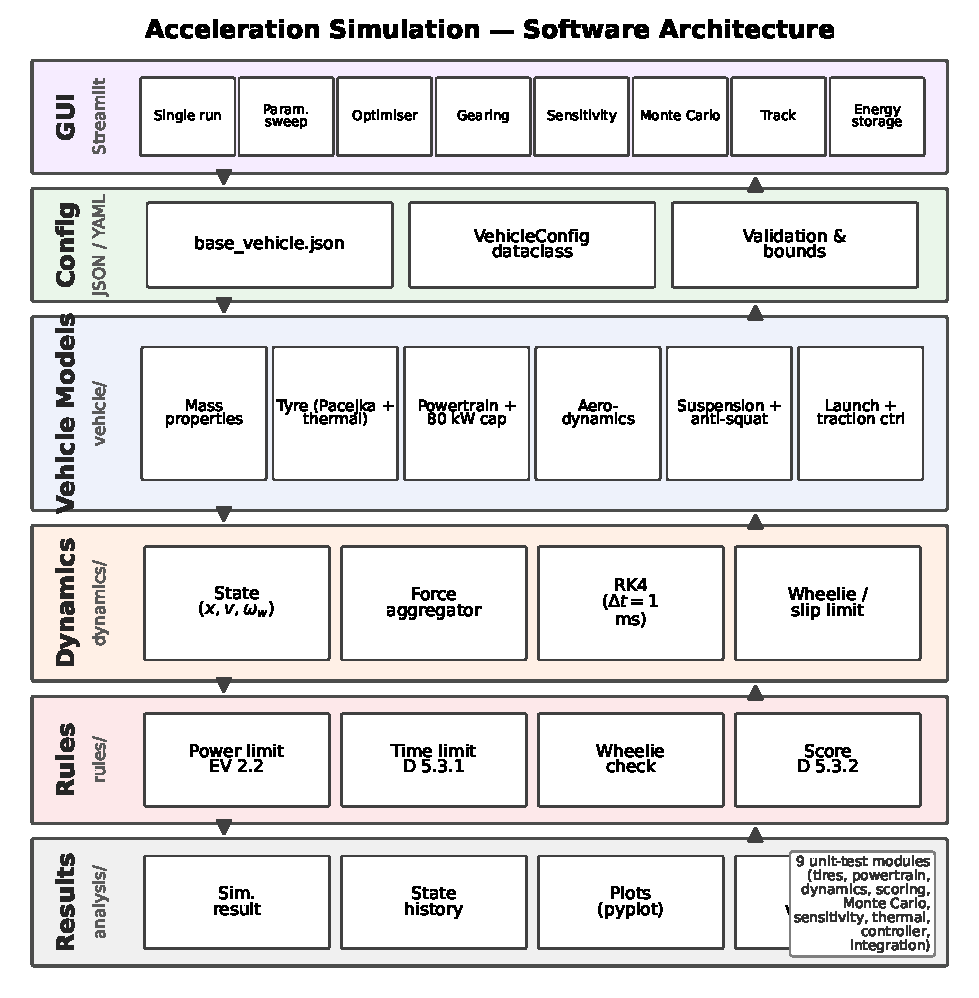
\includegraphics[width=0.95\textwidth]{figures/architecture.pdf}
\caption{Software architecture of the simulation. The five-layer
Python core (Config, Vehicle Models, Dynamics, Rules, Results)
enforces FS-EV~2.2 and FS-D~5.3.1 compliance on every simulated
configuration. A Streamlit-based GUI sits above the core and is used
by the other subsystem chapters to evaluate parameter proposals
interactively.}
\label{fig:architecture}
\end{figure}

% ---------------------------------------------------------------------
\section{Verification and Validation}
\label{sec:vv}
% ---------------------------------------------------------------------

Three checks support the model: a constant-power lower bound
(Section~\ref{sec:analytical_bound}), algebraic spot checks
(Table~\ref{tab:handcalc}), and timestep convergence
(Section~\ref{sec:convergence}).

% ---------------------------------------------------------------------
\subsection{Analytical lower bound}
\label{sec:analytical_bound}
% ---------------------------------------------------------------------

If mass $m$ absorbed constant power $P$ from rest with no drag,
rolling resistance, or traction limit, then
$v(t) = \sqrt{2Pt/m}$ and
$x(t) = \tfrac{2}{3}\sqrt{2P/m}\,t^{3/2}$. At $x=d=\SI{75}{\metre}$,

\begin{equation}
t_\text{cp} = \left(\frac{d}{\tfrac{2}{3}\sqrt{2P/m}}\right)^{2/3}.
\label{eq:analytical_bound}
\end{equation}

For $m=\SI{250}{\kilo\gram}$ and $P=\SI{80}{\kilo\watt}$,
Eq.~\ref{eq:analytical_bound} gives $t_\text{cp}=\SI{2.70}{\second}$
versus \SI{3.78}{\second} from the full simulator. The gap is dominated
by traction-limited launch (including phases below the electrical power
ceiling); drag and drivetrain losses are secondary, and rolling
resistance is negligible at this distance (Section~\ref{sec:tornado}).

% ---------------------------------------------------------------------
\subsection{Analytical hand-calculation agreement}
\label{sec:handcalc}
% ---------------------------------------------------------------------

Table~\ref{tab:handcalc} compares closed-form estimates with the code for
rolling resistance and sustaining power at \SI{20}{\metre\per\second},
unramped launch acceleration at the torque cap, and the wheelie limit
from Eq.~\ref{eq:wheelie}. Peak simulated acceleration stays
\SI{37}{\percent} below wheelie onset (Section~\ref{sec:final_run}).

\begin{table}[H]
\centering
\caption{Algebraic checks vs.\ simulation (launch differs due to the
\SI{80}{\milli\second} ramp in Section~\ref{sec:launch}).}
\label{tab:handcalc}
\footnotesize
\setlength{\tabcolsep}{4pt}
\begin{tabularx}{\textwidth}{|>{\raggedright\arraybackslash\hsize=1.55\hsize}X|c|c|>{\raggedright\arraybackslash\hsize=0.45\hsize}X|}
\hline
\textbf{Quantity} & \textbf{Hand calc.} & \textbf{Simulation} & \textbf{Comment} \\
\hline
Rolling resistance at \SI{20}{\metre\per\second} (\si{\newton})
  & 24.5 & 24.5 & Exact; same $C_\text{rr}$. \\
Power to sustain \SI{20}{\metre\per\second} (\si{\watt})
  & 490 & 490 & Exact. \\
Launch accel., unramped cap (\si{\metre\per\second\squared})
  & 15.76 & 12.66 & Sim: \SI{80}{\milli\second} ramp. \\
Wheelie-limit accel.\ (\si{\metre\per\second\squared})
  & 20.51 & $\ge 12.86$ (no wheelie) & Margin \SI{37}{\percent}. \\
\hline
\end{tabularx}
\end{table}

% ---------------------------------------------------------------------
\subsection{Numerical convergence with timestep}
\label{sec:convergence}
% ---------------------------------------------------------------------

Table~\ref{tab:dt_convergence} lists $t_{75}$ for a coarse timestep, the
adopted $\Delta t=\SI{1}{\milli\second}$, and a fine reference at
\SI{0.2}{\milli\second}. At \SI{1}{\milli\second}, $t_{75}$ differs by
\SI{3}{\milli\second} (\SI{0.08}{\percent}) from the reference---roughly
two orders of magnitude below the $\pm10\,\%$ single-parameter
sensitivities in Section~\ref{sec:tornado}, so discretisation error is
negligible next to modelling uncertainty.

\begin{table}[H]
\centering
\caption{$t_{75}$ vs.\ timestep (reference: $\Delta t=\SI{0.2}{\milli\second}$).}
\label{tab:dt_convergence}
\footnotesize
\begin{tabular}{|c|c|c|}
\hline
$\Delta t$ (ms) & $t_{75}$ (s) & Deviation from ref.\ (ms) \\
\hline
5.00 & 3.825 & $+45.6$ \\
1.00 & 3.782 & $+2.6$ \\
0.20 & 3.779 & $0.0$ \\
\hline
\end{tabular}
\end{table}

% ---------------------------------------------------------------------
\section{Parameter Sensitivity and Design Optimisation}
\label{sec:sensitivity}
% ---------------------------------------------------------------------

The purpose of this section is twofold: to rank the vehicle
parameters by their influence on the \SI{75}{\metre} time
(Section~\ref{sec:tornado}), providing the target ranges used by the
neighbouring chapters; and to report the outcome of a numerical
optimisation over the design vector
(Section~\ref{sec:optimisation}). A short robustness analysis
against track surface conditions closes the section
(Section~\ref{sec:drywet}).

% ---------------------------------------------------------------------
\subsection{One-at-a-time sensitivity ranking}
\label{sec:tornado}
% ---------------------------------------------------------------------

Each candidate design parameter is perturbed by $\pm 10\,\%$ about the
baseline configuration, holding all others fixed, and the change in
predicted \SI{75}{\metre} time is recorded.
Figure~\ref{fig:tornado} shows the resulting tornado plot; dominant
parameters are longitudinal CG and peak tyre grip, with wheel radius,
drivetrain efficiency, mass, and gear ratio forming a second tier (see
caption).

\begin{figure}[H]
\centering

\includegraphics[width=0.85\textwidth]{figures/tornado.pdf}
\caption{One-at-a-time sensitivity of the \SI{75}{\metre} time to a
$\pm 10\,\%$ perturbation of each vehicle parameter. Centre-of-gravity
longitudinal position and tyre peak grip dominate; drivetrain
efficiency, gear ratio, mass and wheel radius form a second band;
aerodynamic drag and rolling resistance are negligible over
\SI{75}{\metre}.}
\label{fig:tornado}
\end{figure}

The ranking has two practical consequences. First, the two dominant
levers (longitudinal CG and tyre peak grip) sit in different subsystems
and cannot both be improved in isolation: shifting the accumulator forward
to reduce $L_{CG}$ couples to mechanical packaging
(Section~\ref{sec:mechanical_design_packaging}), and raising peak grip is
constrained by tyre availability and budget within the suspension and
wheel package (Section~\ref{sec:suspension_requirements}). Second, the aerodynamic and
rolling-resistance contributions are sufficiently small that
investment in either is better deployed on mass or driveline
efficiency.

% ---------------------------------------------------------------------
\subsection{Monte Carlo robustness}
\label{sec:monte_carlo}
% ---------------------------------------------------------------------

A 500-sample Monte Carlo run was performed to quantify the
robustness of the predicted \SI{75}{\metre} time to realistic
parametric uncertainty. Each sample draws total vehicle mass
($\sigma = \SI{8}{\kilo\gram}$), peak tyre grip
($p_{Dx1}$, $\sigma = 6\,\%$), longitudinal and vertical
centre-of-gravity positions
($\sigma = \SI{30}{\milli\metre}$ and \SI{15}{\milli\metre}),
drivetrain efficiency ($\sigma = 1.5\,\%$), and drag area
($\sigma = \SI{0.05}{\metre\squared}$) from independent Gaussians
around the baseline. The results are summarised in
Figure~\ref{fig:mc_histogram}.

\begin{figure}[H]
\centering
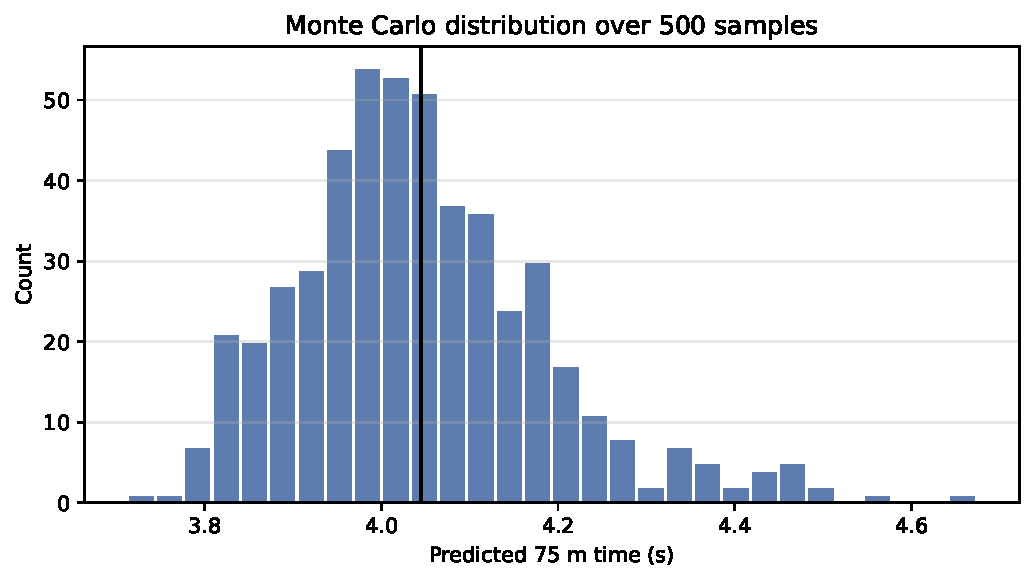
\includegraphics[width=0.82\textwidth]{figures/mc_histogram.pdf}
\caption{Distribution of predicted \SI{75}{\metre} time over
\num{500} Monte Carlo samples using the Gaussian parameter draws
described above.}
\label{fig:mc_histogram}
\end{figure}

Figure~\ref{fig:mc_histogram} summarises the sample distribution:
mean \SI{4.03}{\second} (standard deviation
\SI{120}{\milli\second}), with the 5--95 percentile band
\SIrange{3.86}{4.27}{\second}. The mean sits above the deterministic
baseline \SI{3.78}{\second} and the histogram is positively skewed:
unfavourable draws (lower grip, higher mass, higher CG) cost more time
than favourable draws recover, matching the convex response already seen
in Section~\ref{sec:tornado}. Every sample remained compliant with
FS-EV~2.2 and FS-D~5.3.1 ($t_{75} < \SI{25}{\second}$) with no wheelie
($\min F_{z,f} > 0$), indicating substantial margin across the sampled
envelope.

% ---------------------------------------------------------------------
\subsection{Design optimisation}
\label{sec:optimisation}
% ---------------------------------------------------------------------

The sensitivity ranking above identifies which levers matter but does
not resolve their optimal combination: several are coupled (gear
ratio and wheel radius through the driveline, CG position and
wheelbase through packaging, mass and grip through vertical load).
A formal optimisation is therefore performed over the seven
independent decision variables listed in
Table~\ref{tab:optim_setup}, with the remaining parameters held at
their hardware-pinned values (motor, inverter, supercapacitor pack,
FS rule limits).

\begin{table}[H]
\centering
\caption{Optimisation setup: seven decision variables with physically
motivated bounds. All other vehicle parameters are held at
hardware-pinned values corresponding to the YASA P400R motor, BAMOCAR
PG-D3 inverter, and \num{200}-cell supercap stack
\cite{bamocar_pg, yasa_p400r}.}
\label{tab:optim_setup}
\footnotesize
\begin{tabular}{|l|c|c|l|}
\hline
\textbf{Variable} & \textbf{Baseline} & \textbf{Bounds} & \textbf{Rationale} \\
\hline
Wheelbase $L$ (\si{\metre})               & 1.60 & [1.525, 1.75] & FS-T~2.9.1 min; packaging upper. \\
CG fraction $L_{CG}/L$                    & 0.71 & [0.50, 0.88] & RWD grip vs steering balance. \\
Gear ratio $N_g$                          & 5.5 & [3.0, 7.0] & Drivetrain chapter packaging. \\
Wheel radius $r_w$ (\si{\metre})          & 0.247 & [0.20, 0.28] & 10-inch vs 13-inch rim options. \\
Pacejka $\kappa_\text{opt}$               & 0.14 & [0.08, 0.20] & Slick tyre literature range. \\
Launch torque limit (\si{\newton\metre})  & 1000 & [400, 1200] & YASA peak torque. \\
Anti-squat $\text{AS}$                    & 0.12 & [0.00, 1.00] & Section~\ref{sec:antisquat_dynamic_toe}. \\
\hline
\end{tabular}
\end{table}

The objective is the predicted \SI{75}{\metre} time subject to three
constraints enforced by the Rules layer: FS-EV~2.2 (peak electrical
power $\leq \SI{80}{\kilo\watt}$), FS-D~5.3.1 (finish time
$< \SI{25}{\second}$), and no wheelie
($\min F_{z,f} > 0$). The constraints are baked into the simulation
(configurations that violate them return their full time but are
reported as non-compliant), so the optimiser can use an unconstrained
algorithm. SciPy's Nelder--Mead optimiser \cite{press2007} minimises \(t_{75}\) by
trying new parameter sets and comparing simulated times---no
derivatives---which suits a model with hard limits and FS rule logic;
only seven parameters are tuned.

Figure~\ref{fig:optim_convergence} shows the objective convergence
over the first \num{243} evaluations. The best feasible time
decreases monotonically from the \SI{3.78}{\second} baseline; wheelie-violating
candidates appear as red crosses and are rejected via the objective penalty.
The search converges to
\textbf{\SI{3.67}{\second}} — a \SI{2.9}{\percent} improvement —
with the parameter set shown in Table~\ref{tab:optim_result}. All
three constraints are satisfied at the optimum, and the minimum
front normal force remains comfortably positive.

\begin{figure}[H]
\centering
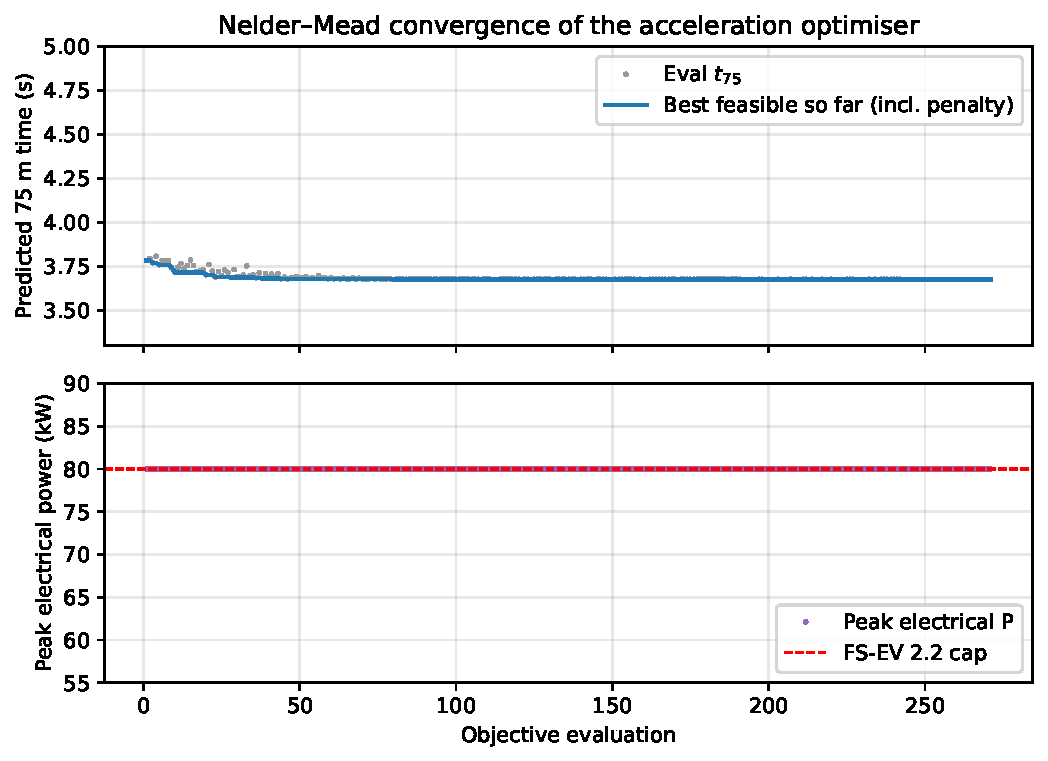
\includegraphics[width=0.82\textwidth]{figures/optim_convergence.pdf}
\caption{Convergence of the Nelder--Mead optimiser over \num{243}
objective evaluations: evaluated \SI{75}{\metre} time (grey dots),
best-so-far curve (blue), and wheelie-violating evaluations (red crosses,
penalised in the objective).}
\label{fig:optim_convergence}
\end{figure}

\begin{table}[H]
\centering
\caption{Optimisation result. The converged design moves the CG
forward relative to the baseline, tightens the gear ratio and
increases anti-squat, and chooses a modestly smaller wheel radius.
The launch torque cap is reduced to prevent the tyre from spinning
through the Pacejka peak.}
\label{tab:optim_result}
\footnotesize
\begin{tabular}{|l|c|c|c|}
\hline
\textbf{Variable} & \textbf{Baseline} & \textbf{Optimised} & \textbf{Change} \\
\hline
Wheelbase $L$ (\si{\metre})      & 1.60 & 1.60 & -- \\
CG fraction $L_{CG}/L$           & 0.71 & 0.63 & $-11\,\%$ \\
Gear ratio $N_g$                 & 5.5 & 4.94 & $-10\,\%$ \\
Wheel radius $r_w$ (\si{\metre}) & 0.247 & 0.227 & $-8\,\%$ \\
Pacejka $\kappa_\text{opt}$      & 0.140 & 0.132 & $-6\,\%$ \\
Launch torque (\si{\newton\metre}) & 1000 & 721 & $-28\,\%$ \\
Anti-squat $\text{AS}$            & 0.12 & 0.36 & $+200\,\%$ \\
\hline
\textbf{\SI{75}{\metre} time (\si{\second})} & \textbf{3.78} & \textbf{3.67} & $\mathbf{-2.9\,\%}$ \\
\hline
\end{tabular}
\end{table}

The optimiser's choices are physically interpretable: the CG shift
forward and the anti-squat increase together preserve front normal
force despite the reduced launch torque cap (which itself prevents
the wheels from spinning through the Pacejka peak); the smaller
wheel and tighter gear ratio increase tractive force at the cost of
top speed, but the extra top-speed margin is not needed over
\SI{75}{\metre}. These results feed back to the neighbouring
chapters as the vehicle-level targets summarised in
Section~\ref{sec:final_params}.

% ---------------------------------------------------------------------
\subsection{Robustness to track surface conditions}
\label{sec:drywet}
% ---------------------------------------------------------------------

The acceleration event is run on a specified track, but ambient
conditions vary between rounds. Scaling the Pacejka peak grip by a
surface-condition multiplier (\num{1.0} for dry slicks on clean
tarmac, \num{0.60} for the same slicks on a water film
\cite{milliken1995}) gives a wet-track prediction of
\SI{4.83}{\second} versus \SI{3.78}{\second} dry --- a
\SI{28}{\percent} time penalty (Figure~\ref{fig:drywet}). Both
configurations remain inside the \SI{25}{\second} disqualification
threshold and neither exceeds the \SI{80}{\kilo\watt} power cap,
confirming that the design is rule-compliant across the plausible
track-condition envelope. In wet conditions the phase transition
(Section~\ref{sec:constraint_activity}) shifts later in the run: the
vehicle spends more of the event traction-limited and less of it
power-limited, which is consistent with the reduced grip ceiling at
every velocity.

\begin{figure}[H]
\centering
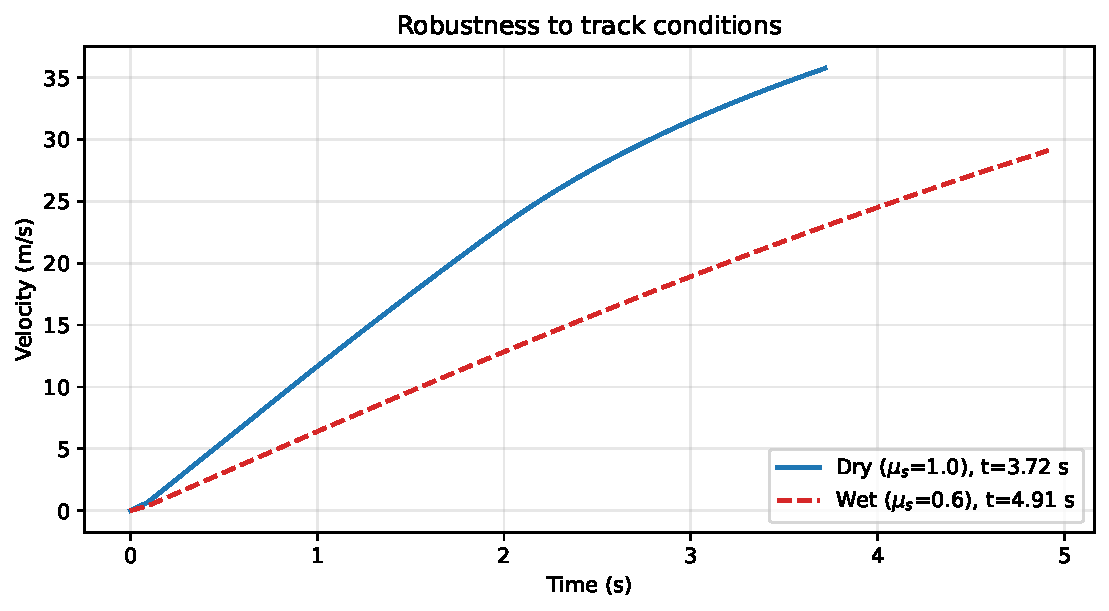
\includegraphics[width=0.8\textwidth]{figures/dry_wet.pdf}
\caption{Velocity trace under dry and wet surface conditions (peak
grip multiplier \num{1.0} vs \num{0.60}). The \SI{28}{\percent} time
penalty on wet tracks is dominated by the extended traction-limited
phase; both configurations remain compliant with FS-EV~2.2 and
FS-D~5.3.1.}
\label{fig:drywet}
\end{figure}

% ---------------------------------------------------------------------
\section{Predicted Performance of the Final Vehicle}
\label{sec:final_run}
% ---------------------------------------------------------------------

The final agreed vehicle configuration combines decisions across the
Chassis, Suspension, Drivetrain, and Supercapacitors chapters. The
simulation takes the finalised configuration as input and produces
predicted performance traces together with checks against FS-EV~2.2,
FS-D~5.3.1, and pitch stability.

% ---------------------------------------------------------------------
\subsection{Final agreed parameter set}
\label{sec:final_params}
% ---------------------------------------------------------------------

\begin{table}[H]
\centering
\caption{Final agreed parameter set: principal inputs matching the
longitudinal simulation baseline (Section~\ref{sec:monte_carlo},
Table~\ref{tab:pacejka}), with electrical hardware figures from the
Drivetrain and Supercapacitors chapters.}
\label{tab:final_parameters}
\footnotesize
\begin{tabular}{|l|c|c|l|}
\hline
\textbf{Parameter} & \textbf{Symbol} & \textbf{Value} & \textbf{Source} \\
\hline
Total vehicle mass & $m_v$ & 200\si{\kilo\gram} & Section~\ref{sec:monte_carlo}; chassis $<$\SI{220}{\kilo\gram} \\
Wheelbase & $L$ & 1.60\si{\metre} & Chassis \\
CG longitudinal & $L_{CG}$ & 1.14\si{\metre} & Section~\ref{sec:load_transfer} \\
CG height & $h_{CG}$ & 0.22\si{\metre} & Section~\ref{sec:load_transfer} \\
Wheel radius & $r_w$ & 0.247\si{\metre} & Section~\ref{sec:monte_carlo}; loaded radius \\
Peak tyre grip & $p_{Dx1}$ & 1.70 & Table~\ref{tab:pacejka} \\
Accumulator nominal voltage & $V_\text{bus}$ & 600\si{\volt} & Supercapacitors \\
Accumulator mass & $m_\text{acc}$ & 27.8\si{\kilo\gram} & Supercapacitors \\
Motor torque constant & $K_t$ & 0.822\si{\newton\metre\per\ampere} & Drivetrain (YASA P400R) \\
Motor peak RMS current & $I_m^\text{peak}$ & 285\si{\ampere} & Drivetrain (BAMOCAR PG-D3) \\
Gear ratio & $N_g$ & 5.5 & Section~\ref{sec:powertrain} \\
Drivetrain efficiency & $\eta_\text{drv}$ & 0.95 & Section~\ref{sec:powertrain} \\
Drag area & $C_d A$ & 0.80\si{\metre\squared} & Chassis \\
Anti-squat ratio & $\text{AS}$ & 0.36 & Section~\ref{sec:monte_carlo}; geometry Section~\ref{sec:antisquat_dynamic_toe} \\
\hline
\end{tabular}
\medskip

\noindent\footnotesize\textit{Note.}
The runnable simulation configuration contains many further parameters
(for example full tyre coefficients, launch-controller timings, and
numerical settings); Table~\ref{tab:final_parameters} lists only the
main quantities needed for cross-chapter integration.
\end{table}

% ---------------------------------------------------------------------
\subsection{Constraint activity and phase analysis}
\label{sec:constraint_activity}
% ---------------------------------------------------------------------

Figure~\ref{fig:final_run} shows the predicted four-channel trace of
the baseline vehicle, anchoring the numerical discussion while the
final agreed parameters are confirmed. Three features are worth
commenting on explicitly, because they determine where design effort
is most profitably spent.

\begin{figure}[H]
\centering
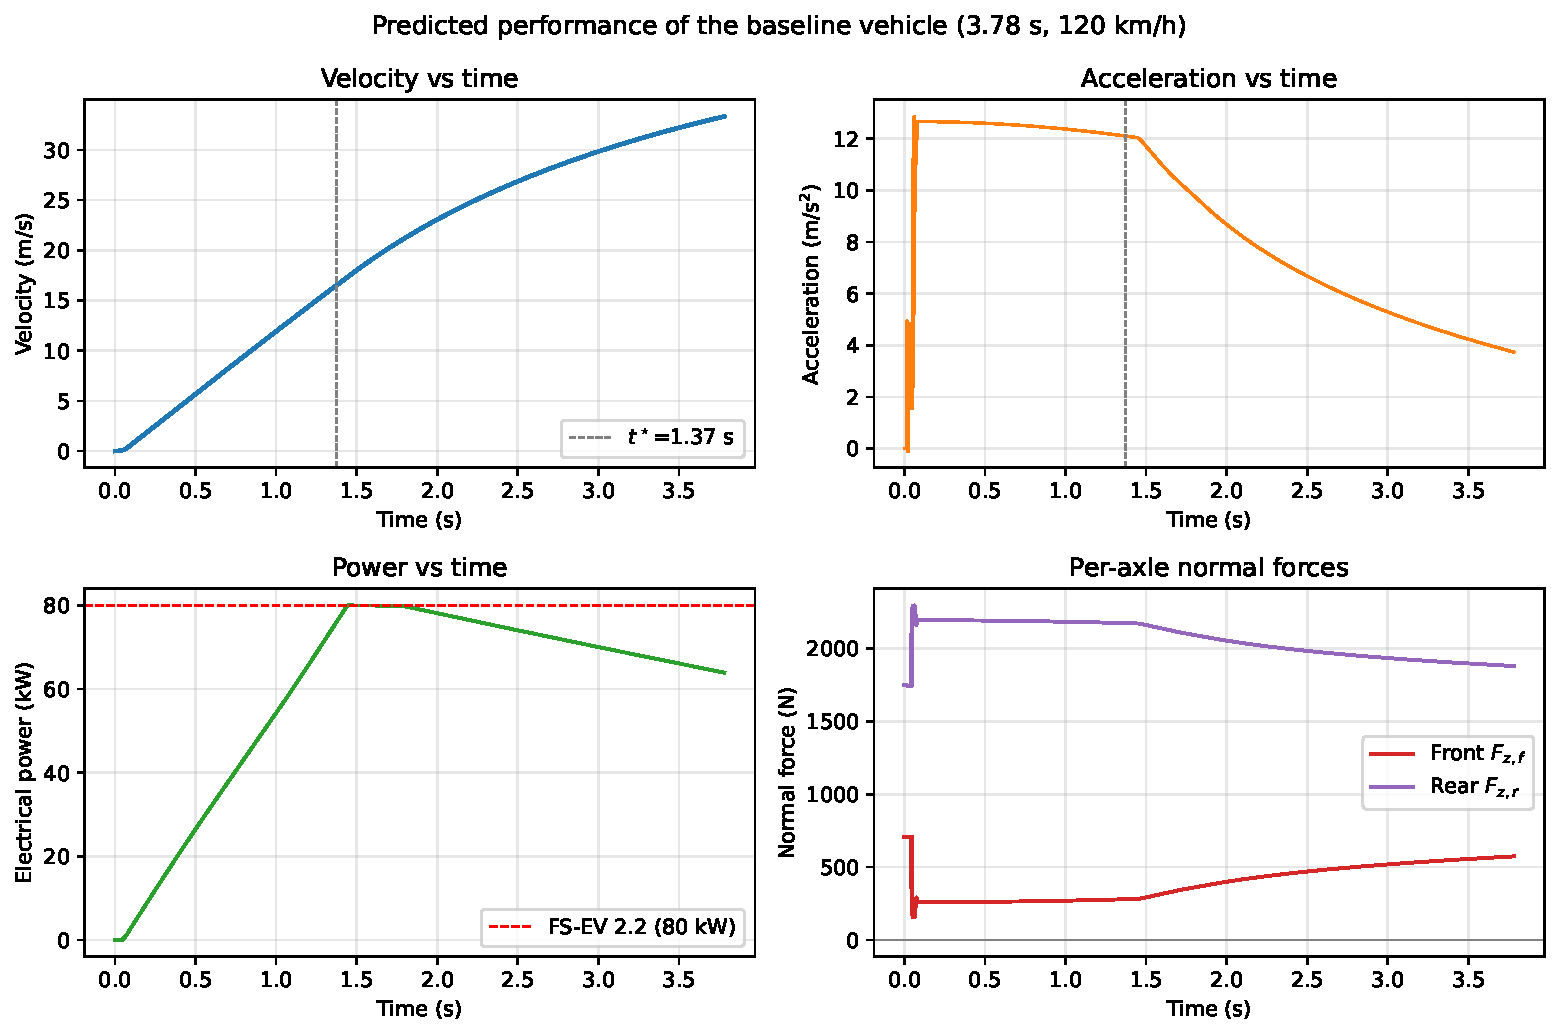
\includegraphics[width=0.95\textwidth]{figures/final_run.pdf}
\caption{Predicted performance of the baseline vehicle. The
grey dashed line at $t^\star = \SI{1.37}{\second}$ marks the
transition from the traction-limited to the power-limited regime.
Instantaneous electrical power (lower left) saturates cleanly at
the FS-EV~2.2 cap, and the front normal force (lower right) remains
positive throughout the run.}
\label{fig:final_run}
\end{figure}

First, the vehicle spends \SI{1.37}{\second} (\SI{36}{\percent} of
the total run time) in the traction-limited regime and
\SI{2.41}{\second} (\SI{64}{\percent}) in the power-limited regime,
with the transition occurring at
$v^\star = \SI{15.4}{\metre\per\second}$ as predicted analytically
in Section~\ref{sec:powertrain}. The grip utilisation during the
traction-limited phase averages approximately \SI{103}{\percent}
relative to the reference Pacejka peak, confirming the launch
controller (Section~\ref{sec:launch}) tracks the load-dependent grip
ceiling closely.

Second, the electrical power saturates cleanly at \SI{79.80}{\kilo\watt}
(against the \SI{80}{\kilo\watt} cap), without overshoot, throughout
the power-limited phase. This is the evidence that
Eq.~\ref{eq:power_limit} is correctly enforced at the electrical
side rather than at the wheel.

Third, the front normal force falls smoothly from a static
\SI{707}{\newton} to a minimum of \SI{158}{\newton} at peak
acceleration and recovers as the vehicle enters the power-limited
phase. The \SI{158}{\newton} minimum is a \SI{22}{\percent} fraction
of the static load, which is ample margin against the wheelie
threshold and validates the choice of anti-squat and CG
geometry for the baseline configuration.

% ---------------------------------------------------------------------
\section{Discussion and Limitations}
\label{sec:discussion}
% ---------------------------------------------------------------------

The simulation is highly detailed and
consistent with the validation evidence in Section~\ref{sec:vv}, but it
omits a few other models that could reduce the gap between sim and reality. Main gaps:
\textbf{driveline torsional compliance} (minor launch oscillation; beyond the rigid torque path implied by Section~\ref{sec:mechanical_design_packaging}),
\textbf{motor electrical dynamics} (finite torque rise time and brief dips; beyond the quasi-static electrical limit in Section~\ref{sec:powertrain}),
\textbf{fixed $V_\text{bus}$} versus supercap voltage sag (Section~\ref{subsec:supercapacitor_analysis} develops pack discharge, which is not yet coupled dynamically here), and \textbf{driver reaction time}
(\SIrange{0.2}{0.4}{\second} omitted). Combined with
Section~\ref{sec:monte_carlo}, the headline \SI{75}{\metre} time is
estimated within roughly $\pm \SI{0.20}{\second}$.

% ---------------------------------------------------------------------
\section{Conclusions and Further Work}
\label{sec:conclusions}
% ---------------------------------------------------------------------

The following conclusions are drawn from the evidence presented in
Sections~\ref{sec:vv}--\ref{sec:discussion}:

\begin{itemize}
    \item Longitudinal simulation with load transfer, Pacejka grip,
          traction-controlled launch, FS-EV~2.2 electrical limiting,
          and RK4 integration at \SI{1}{\milli\second}.
    \item Validated against hand calculations, timestep convergence,
          and an analytical constant-power bound (Section~\ref{sec:vv}).
    \item Dominant sensitivities: longitudinal CG and peak grip;
          secondary band: wheel radius, driveline efficiency, mass,
          gearing (Section~\ref{sec:tornado}).
    \item Optimisation (\num{243} Nelder--Mead evaluations) yields
          \SI{3.67}{\second} versus \SI{3.78}{\second} baseline
          (Section~\ref{sec:optimisation}).
    \item Wet-track scaling remains inside rule limits
          (Section~\ref{sec:drywet}).
    \item Under FS-D~5.3.2 with a notional $T_\text{fastest}=\SI{3.5}{\second}$,
          the baseline predicts \num{59.2}/75 points and the optimised
          set \num{65.1}/75.
\end{itemize}

\subsection*{Further work}

\begin{itemize}
    \item Calibrate Pacejka coefficients from measured longitudinal tyre data.
    \item Couple accumulator voltage sag (Supercapacitors chapter); optionally
          add driveline torsion and motor transient effects.
    \item Re-scope the framework to Skidpad/Autocross if championship score
          trades appear.
\end{itemize}

% ---------------------------------------------------------------------
\compactbib
% ---------------------------------------------------------------------
